\documentclass{article}
\usepackage{color}
\usepackage{amsmath}
\usepackage{graphicx}
\usepackage{geometry}
\usepackage{xcolor}
\geometry{letterpaper, total={170mm,257mm}, left=20mm, top=20mm}
\graphicspath{ {./images/} }
\newcommand{\Lim}[1]{\raisebox{0.5ex}{\scalebox{0.8}{$\displaystyle \lim_{#1}\;$}}}

\title{Vector Calculus}
\author{Justin Bornais}
\date{May 11, 2023}

\begin{document}
\maketitle

\section{Construction of a Line}
\subparagraph{}
The equation of a line is $y=mx+b$, where $y$ is the dependent variable and $x$ is the dependent variable. Now, the equation of a line passing through ($x_0,y_0,z_0$) (or $\vec{r_0}$) and is parallel to the vector $\vec{v}$ is $\vec{r}=\vec{r_0}+t\vec{v}, t\in R$
\section{Planes}
\subparagraph{}
The equation of the plane is $ax+by+cz=d$ where $\vec{n}=<a,b,c>$ is the normal vector of the plane.
\subsection{Cylinders}
A \textbf{cylinder} is a surface that consists of all lines parallel to a line and passing through $a$.
\paragraph[Examples]{Examples: Identify and sketch the surface}
\subparagraph{1. $x^2+y^2=4\rightarrow \text{a circle in 2 dimensions} $}
$x^2+y^2=4$ is a cylinder in 3 dimensions (a surface where one variable is missing is a cylinder, the missing variable is the axis).
\subparagraph{2. $y^2+z^2=9$} A cyliinder with x-axis as the axis.
\subparagraph{3. $z=x^2$} A cylinder with y-axis as the axis.

\section{Quadrics}
A quadric in two dimensions is:
\begin{enumerate}
    \item A parabola $y=x^2$ or $x=y^2$
    \item An ellipse: $\frac{x^2}{a^2}+\frac{y^2}{b^2}=1$
    \item A hyperbola: $\frac{x^2}{a^2}-{y^2}{b^2}=1$
\end{enumerate}
A trace is the curve of the intersection of the surface with the coordinate plane $\rightarrow$ 3 traces.
\newpage
\subsection{Quadric Surface}
$Ax^2+By^2+Cz^2+Dxy+Exz+Fzy+Gx+Hy+Iz+J=0$
\newline In this course, we need to know 6 quadric surfaces.\newline
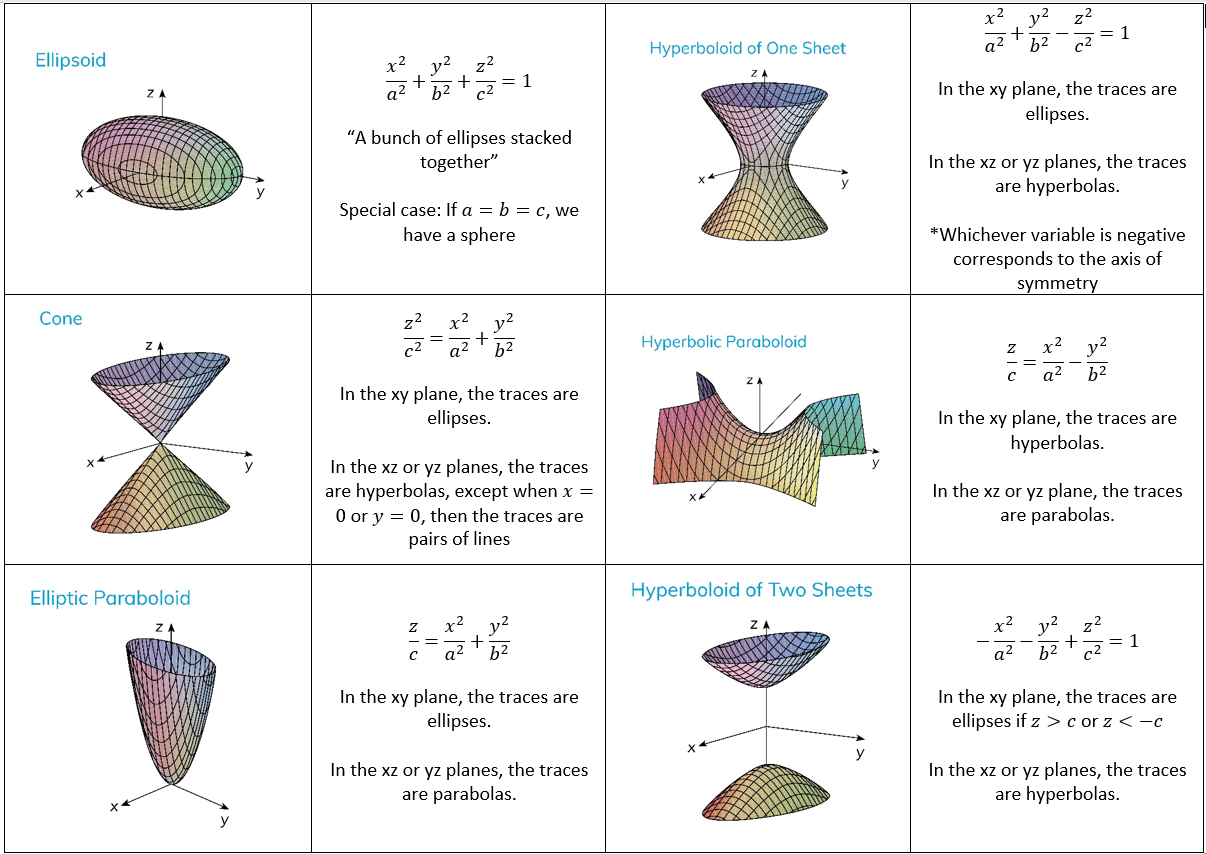
\includegraphics[width=\textwidth]{quadric_surfaces.png}

\paragraph{} We can actually know some patterns for the rest of the quadric surfaces:
\begin{itemize}
    \item \textbf{Ellipsoid} $\Rightarrow \frac{x^2}{a^2}+\frac{y^2}{b^2}+\frac{z^2}{c^2}=1$
    \item \textbf{Hyperboloid of One Sheet} $\Rightarrow \frac{x^2}{a^2}+\frac{y^2}{b^2}-\frac{z^2}{c^2}=1$
    \item \textbf{Hyperboloid of Two Sheets} $\Rightarrow -\frac{x^2}{a^2}-\frac{y^2}{b^2}+\frac{z^2}{c^2}=1$
    \item \textbf{Cone} $\Rightarrow \frac{z^2}{c^2}=\frac{x^2}{a^2}+\frac{y^2}{b^2}$
    \item \textbf{Elliptic Paraboloid} $\Rightarrow  \frac{z}{c}=\frac{x^2}{a^2}+\frac{y^2}{b^2}$
    \item \textbf{Hyperbolic Paraboloid} $\Rightarrow  \frac{z}{c}=\frac{x^2}{a^2}-\frac{y^2}{b^2}$
\end{itemize}
Notice the patterns with the equations?
\newpage
\subsubsection{Elliptic Paraboloids}
The equation of an elliptic paraboloid is $\frac{z}{c}=\frac{x^2}{a^2}+\frac{y^2}{b^2}$ where $z$ is the axis, $xy$ traces are ellipses ($x=0$) and both $\frac{x^2}{a^2}$ and $\frac{y^2}{b^2}$ have the same signs.
\newline \indent 2 traces is a parabola, 1 trace is an ellipse.
\newline\newline Effectively, the variable with a power of $1$ is the axis.
\subparagraph{$z=0$}$\Rightarrow 0=\frac{x^2}{a^2}+\frac{y^2}{b^2} \Rightarrow x=0,y=0,z=0$
\subparagraph{$z=k$}$\Rightarrow \frac{k}{c}=\frac{x^2}{a^2}+\frac{y^2}{b^2} \Rightarrow$ ellipses for $k>0$

\subsubsection{Hyperboloid of One Sheet}
The variable with the negative sign is the axis. The \textbf{xy-trace} is where $z=0$. The \textbf{xz-trace} and \textbf{yz-trace} is a hyperbola.

\subsubsection{Hyperboloid of Two Sheets}
The variable with the positive sign is the axis. The \textbf{xy-trace} is an ellipses if $\lvert z \rvert > \lvert c \rvert $

\subsubsection{Cone}
The variable with the negative sign is the axis. Two traces are hyperbolas, one trace is an ellipse for $k\ne 0$.

\subsubsection[Exampls]{Examples: Identify and sketch the surfaces}
\paragraph{1. $x^2+4y^2+z^2=4$} $\Rightarrow \frac{x^2}{4}+\frac{y^2}{4}+\frac{z^2}{4}=1$
\paragraph{3. $z^2=x^2+4y^2+64$} $\Rightarrow -x^2-4y^2+z^2=64$
$\Rightarrow -\frac{x^2}{64}-\frac{y^2}{16}+\frac{z^2}{64}=1$ (hyperboloid on 2 sheets, axis is z-axis with $c=8$)

\newpage
\section{Vector Functions}
These are chapters 13.1 and 13.2 from last class.

A vector function is $\vec{r}(t)=<f(t),g(t),h(t)>$ such that $f(t)=x$, $g(t)=y$ and $h(t)=z$.
\begin{itemize}
    \item For 2 dimensions: $\vec{r}(t)=<f(t),g(t)>$
    \item $\vec{r}\,'(t)=<f'(t),g'(t)>$ or $\vec{r}\,'(t)=<f'(t),g'(t),h'(t)>$
\end{itemize}

\subsection{Arc Length}
The equation for length is $|\vec{r}\,'(t)|=\sqrt{(f'(t))^2+(g'(t))^2}$ for 2 dimensions,
or $|\vec{r}\,'(t)|=\sqrt{(f'(t))^2+(g'(t))^2+(h'(t))^2}$ for 3 dimensions.

Now, the formula is effectively $\sqrt{(\delta x)^2 + (\delta y)^2}$, where $x=f(t)$ and $\delta x=f'(t)dt$ and similarly for $y$.
\\Thus the formula is $\sqrt{(f'(t)dt)^2+(g'(t)dt)^2}=\sqrt{(f'(t))^2+(g'(t))^2(dt)^2}=\sqrt{(f'(t))^2+(g'(t))^2}dt$
\\\\\textbf{Arc Length is: } $L=\int_{a}^{b} \sqrt{(f'(t))^2+(g'(t))^2}dt$
\\Thus, the arc length of a curvee $\vec{r}(t)$ for $a\leq t\leq b$ is $\int_{a}^{b} |\vec{r}\,'(t)|dt$

\subsection{Example 1}
Find the length of the curve $\vec{r}(t)=<2\sin^3t,2cos^3t>, 0\leq t\leq \frac{\pi}{4}$
\\\\\textbf{Solution:} $\vec{r} '(t)=<2(3\sin^2t)(\cos t), 2(3\cos^2t)(-\sin t)>$
\\$|\vec{r}\,'(t)|=\sqrt{(6sin^2t \cos t)^2+(-6\cos^2t \sin t)^2}$
\\$=\sqrt{36\sin^4t \cos^2t+36\cos^4t\sin^2t}$
\\$=\sqrt{36\sin^2t\cos^2t(\sin^2t+\cos^2t)}$
\\$=\sqrt(36\sin^2t\cos^2t(1))$
\\$=6\sin t\cos t$
\\\\The arc length $L=\int_{a}^{b} |\vec{r}\,'(t)|dt=\int_{0}^{\frac{\pi}{4}} 6\sin t\cos tdt$
\\Let $u=\sin t$ so $du=\cos tdt$
\\\\Then we have $L=\int_{0}^{\frac{\pi}{4}} 6udu=\frac{6u^2}{2}=3u^2$
\\$=3\sin^2t |_{t=0}^{\frac{\pi}{4}}=3\sin^2\frac{\pi}{4}-3\sin^20=3(\frac{1}{2})=\frac{3}{2}$

\subsection{Example 2}
Find the length of the curve $\vec{r}(t)=<t^2,2t,\ln t>, 1\leq t\leq e$
\\\\\textbf{Solution:} $\vec{r}\,'(t)=<2t,2,\frac{1}{t}>$
\\$|\vec{r}\,'(t)|=\sqrt{4t^2+4+\frac{1}{t^2}}=\sqrt{\frac{4t^4+4t^2+1}{t^2}}=\frac{\sqrt{(2t^2+1)^2}}{\sqrt{t^2}}=\frac{2t^2+1}{t}$
\\$L=\int_{a}^{b} |\vec{r}\,'(t)|dt=\int_{1}^{e} \frac{2t^2+1}{t}dt=\int_{1}^{e} \left(\frac{2t^2}{t}+\frac{1}{t}\right)dt$
\\$L=\int_{1}^{e} \left(2t+\frac{1}{t}\right)dt=t^2+\ln |t|\,\,|_{1}^{e}$
\\$L=e^2+\ln |e|-1^2-\ln 1=e^2$

\newpage
\subsection{Curvature}
In the last class, the unit tangent vector $\vec{T}(t)=\frac{\vec{r}\,'(t)}{|\vec{r}\,'(t)|}$.
Curvature is the magnitude of the rate of change of the unit tangent vector w.r.t. the arc length.
\\\\\textbf{Arc Length Function} $S=\int_{a}^{t}\left|\vec{r}\,'(u) \right|du$
\\\textbf{Curvature Function} $K=\left|\frac{d\vec{T}}{ds}\right|$
\begin{itemize}
    \item Note: $\frac{d\vec{T}}{dt}=\frac{d\vec{T}}{ds}\frac{ds}{dt} \rightarrow$ chain rule.
    \\ $\frac{d\vec{T}}{dt}=\frac{d\vec{T}}{ds}|\vec{r}\,'(t)|\Rightarrow \left|\frac{d\vec{T}}{ds}\right|=\frac{\left|\frac{d\vec{T}}{dt}\right|}{|\vec{r}\,'(t)|}=\frac{|\vec{T}\,'(t)|}{|\vec{r}\,'(t)|}$
    \item Thus $K=\frac{|\vec{T}\,'(t)|}{|\vec{r}\,'(t)|}$
    \item Another formula for $K=\frac{|\vec{r}\,'(t)\times\vec{r}\,''(t)|}{|\vec{r}\,'(t)|^3}$
\end{itemize}

\subsection{Example 1}
Find the curvature of the following curve: $\vec{r}(t)=<5\sin t,3t, 5\cos t>$
\\\\\textbf{Solution:} $\vec{r}\,'(t)=<5\cos t,3,-5\sin t>$, $|\vec{r}\,'(t)=\sqrt{25\cos^2t+9+25\sin^2t}=\sqrt{25(\cos^2t+\sin^2t)+9}=\sqrt{34}$
\\$\vec{T}(t)=\frac{\vec{r}\,'(t)}{|\vec{r}\,'(t)}=\frac{<5\cos t,3,-5\sin t>}{\sqrt{34}}$
\\$\vec{T}\,'(t)=\frac{1}{\sqrt{34}}<-5\sin t,0,-5\cos t>$
\\$\left|\vec{T}\,'(t)\right|=\sqrt{\frac{1}{34}\left(25\sin^2t+25\cos^2t\right)}=\sqrt{\frac{25}{34}}=\frac{\frac{5}{\sqrt{34}}}{\sqrt{34}}$ (divide by $\sqrt{34}$ one more time since we're trying to find $K$)

\subsection{Example 2}
Find the curvature of the following curve: $\vec{r}\,'(t)=<t,t,1+t^2>$
\\\\\textbf{Solution:} $\vec{r}\,'(t)=<1,1,2t>$, $|\vec{r}\,'(t)|=\sqrt{1^2+1^2+4t^2}=\sqrt{2+4t^2}
\\\vec{T}\,'(t)=\frac{\vec{r}\,'(t)}{|\vec{r}\,'(t)}=\frac{<1,1,2t>}{\sqrt{2+4t^2}}=\left<\frac{1}{\sqrt{2+4t^2}},\frac{1}{\sqrt{2+4t^2}},\frac{2t}{\sqrt{2+4t^2}} \right>$
\\$\vec{T}\,'(t)=...$ (hard to calculate)
\\\textbf{Instead, another formula for K:} $K=\frac{|\vec{r}\,'(t)\times\vec{r}\,''(t)|}{|\vec{r}\,'(t)|^3}$
\\$\vec{r}\,''(t)=<0,0,2>$
\\$\vec{r}\,'(t)\times\vec{r}\,''(t)=\begin{bmatrix}
    \hat{i} & \hat{j} & \hat{k} & \\
    1 & 1 & 2t \\
    0 & 0 & 2
\end{bmatrix}=\hat{i}(2-0)-\hat{j}(2-0)+\hat{k}(0-0)=2\hat{i}-2\hat{j}+0\hat{k}\;or\;<2,-2,0>$ (remember cross product in MATH1250)
\\$K=\frac{|\vec{r}\,'(t)\times\vec{r}\,''(t)|}{|\vec{r}^3|}=\frac{\sqrt{8}}{\left(\sqrt{2+4t^2}\right)^3}$
\newpage

\section{(13.4) Motion in Space}
We learned that $\vec{r}(t)=<f(t),g(t),h(t)>$ where $f(t)=x$, $g(t)=y$ and $h(t)=z$.
\begin{itemize}
    \item If the position vector/function of an object is $\vec{r}(t)=<f(t),g(t),h(t)>$ then the velocity of the object is $\vec{v}(t)=\vec{r}\,'(t)$ and it will be in the direction of the tangent vector $\vec{r}\,'(t)$.
    \item The speed is $\left|\vec{v}(t)\right|=\left|\vec{r}\,'(t)\right|$
    \item The acceleration of the object is $\vec{a}(t)=\vec{v}\,'(t)=\vec{r}\,''(t)$
\end{itemize}

\subsubsection{Example 1}
Find the velocity, acceleration and speed of a particle with position vector (function) $\vec{r}(t)=<e^t,t^4,e^{-t}>$

\paragraph{Solution} $\vec{v}(t)=\vec{r}\,'(t)=<e^t,4t^3,-e^{-t}>\;\rightarrow\text{velocity}$
\\Acceleration is $\vec{a}(t)=\vec{v}\,'(t)=<e^t,12t^2,e^{-t}>$
\\Speed is $|\vec{v}(t)|=\sqrt{\left(e^t\right)^2+\left(4t^3\right)^2+\left(e^{-t}\right)}=\sqrt{e^{2t}+16t^6+e^{-2t}}$


\subsubsection{Example 2}
Find the velocity, acceleration and speed of a particle with position vector $\vec{r}(t)=<e^t,t^4,e^{-t}>$ at $t=0$.

\paragraph{Solution} From example 1, $\vec{v}(t)=<e^t,4t^3,-e^{-t}>$
\\At $t=0$, the velocity is $\vec{v}(0)=<e^0,4(0)^3,-e^{-0}>=<1,0,-1>$
\\The speed at $t=0$ is $\sqrt{1^2+0^2+(-1)^2}=\sqrt{2}$
\\$\vec{a}(t)=<e^t,12t^2,e^{-t}>$
\\At $t=0$, $\vec{a}(0)=<e^0,12(0)^2,e^{-0}>=<1,0,1>$

\subsubsection{Example 3}
Given the acceleration vector $\vec{a}(t)=<2t,1,t^2>$ amd the initial velocity is $\vec{v}(0)=<0,1,1>$
and the initial position vector is $\vec{r}(0)=<2,0,-1>$, find the velocity and position vectors of the particle.

\paragraph{Solution}
The velocity is $\vec{v}(t)=\int \vec{a}(t)dt=\int <2t,1,t^2>dt
\\=<\frac{2t^2}{2}+C_1,t+C_2,\frac{t^3}{3}+C_3>\;\text{or }<t^2,t,\frac{t^3}{3}>+<C_1,C_2,C_3> (\vec{C})$
\\$\vec{v}(0)=<0,1,1>\Rightarrow<0,1,1>=<0+C_1,0+C_2,0+C_3>\Rightarrow C_1=0, C_2=1, C_3=1$
\\Thus the velocity is $\vec{v}(t)=<t^2,t+1,\frac{t^3}{3}+1>$
\\\\The position vector is $\vec{r}(t)=\int \vec{v}(t)dt=\int<t^2,t+1,\frac{t^3}{3}+1>dt$
\\$\vec{r}(t)=<\frac{t^3}{3}+d_1,\frac{t^2}{2}+t+d_2,\frac{t^4}{12}+t+d_3>$
\\$\vec{r}(0)=<2,0,-1>\Rightarrow<2,0,-1>=<0+d_1,0+d_2,0+d_3>\Rightarrow d_1=2,d_2=0,d_3=-1$
\\So $\vec{r}(t)=<\frac{t^3}{3}+2,\frac{t^2}{2}+t,\frac{t^4}{12}+t-1>$

\section{Functions of Several Variables (or Multivariable Functions)}
\textbf{Multivariable Functions} are functions with at least 2 independent variables.
In \textbf{chapters 14 and 15}, we cover domains, limits, continuity, derivatives
and applications, integration and applications. \begin{itemize}
    \item One prominent example is the volume functions $V=xyz$ and $V=\pi r^2h$
\end{itemize}

\subsection{Functions of 2 Variables}
$x$ and $y$ are independent variables, and the domain will be in $R^2$:
$D=\{(x,y)\;|\;\text{properties}\}$
\\A function in 2 variables, $z=f(x,y)$ is a rule that assigns to each $(x,y)\in D$ a unique value $z$ in $R$.
\begin{itemize}
    \itemsep 0em
    \item The domain $D$ is $R^2$ (inputs).
    \item The range is a subset of $R$ (outputs).
    \item $z=f(x,y)\rightarrow\;\text{explicit.}$
    \item $f(x,y,z)=0\rightarrow\;\text{implicit.}$
\end{itemize}

The vertical line test (VLT) can be used to check if a single-variable relation is a function.
This is similar for 2-variable functions, the VLT will instead draw lines parallel to the z-axis.
The relation will be a function if every vertical line crosses the surface of a function only once.

\subsubsection{Example 1}
Find the domain of $f(x,y)=\ln(x+y)$
\paragraph{Solution} We need $x+y>0\Rightarrow y>-x$
\\Thus the domain of $f=\{(x,y)\;|\;y>-x\}$

\subsubsection{Example 2}
Find the domain of $f(x,y)=\sqrt{1+x-y^2}$

\paragraph{Solution} We need $1+x-y^2\geq0\Rightarrow x\geq y^2-1$
\\Thus the domain of $f=\{(x,y)\;|\;x\geq y^2-1\}$

\subsection{Sketch the Domains}
Draw $x=y^2-1$\\
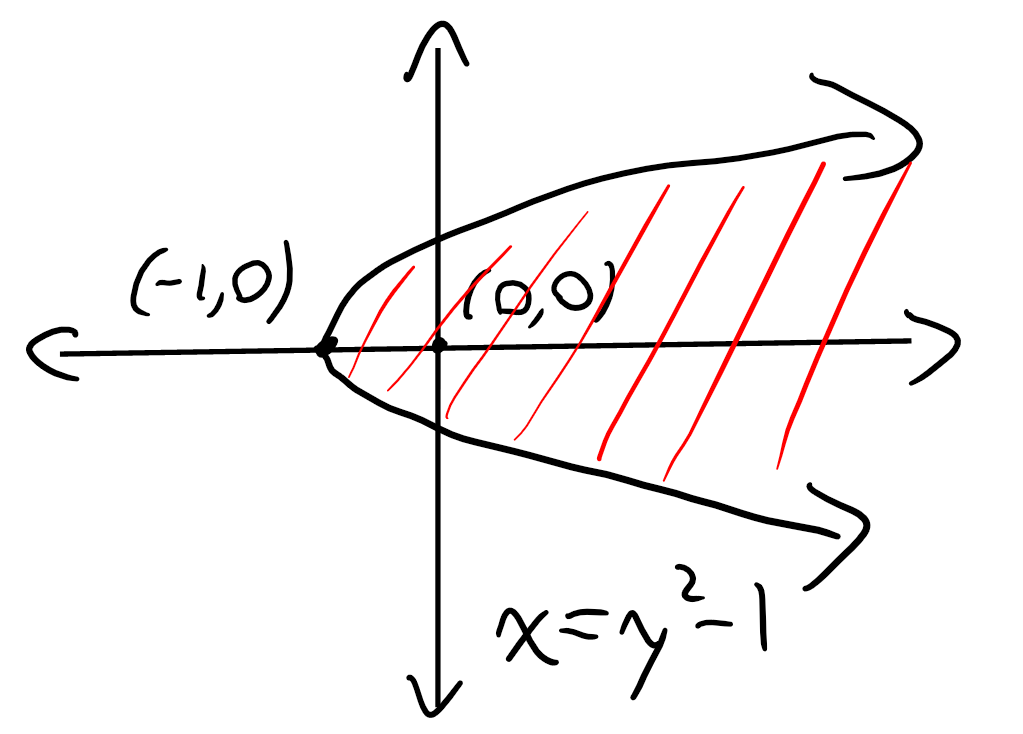
\includegraphics[width=200px]{sketch-domain.png}
\\Choose a test point, (0,0)
\\$x\geq y^2-1\Rightarrow0\geq0-1\Rightarrow0\geq-1\;\text{True}\Rightarrow \text{Shade the side that has (0,0)}$
\\Graphing the surface $z=f(x,y)$ will be in 3 dimensions.

\subsubsection{Example 1}
Sketch the graph of the following function: $f(x,y)=8-x-2y$

\paragraph{Solution} $z=8-x-2y\Rightarrow x+2y+z=8\Rightarrow\;\text{a plane}$
\\x-intercept: $y=0,z=0\Rightarrow x=8\Rightarrow(8,0,0)$
\\y-intercept: $x=0,z=0\Rightarrow 2y=8\Rightarrow y=4\Rightarrow(0,4,0)$
\\z-intercept: $x=0,y=0\Rightarrow z=8\Rightarrow(0,0,8)$

\subsubsection{Example 2}
Sketch the graph of the following function: $f(x,y)=\sqrt{2x^2+y^2}$

\paragraph{Solution} $z=\sqrt{2x^2+y^2}\Rightarrow z^2=2x^2+y^2\Rightarrow 2x^2+y^2-z^2=0\Rightarrow\;\text{a cone}$

\subsubsection{Example 3}
Sketch the graph of the following function: $f(x,y)=-\sqrt{2x^2+y^2}$

\newpage\subsection{(14.1) Functions}
In last class, we did functions of 2 variables, such as $z=f(x,y)$ where $(x,y)\in D$ where $D$ is the domain in $R^2$.
However, this idea can be extended to more than 2 variables. A 3-variable function would have $w=f(x,y,z)$ (explicit form) or $f(x,y,z,w)=0$ (implicit form).

\subsubsection{Example}
Find the domain of $f(x,y,z)=\frac{1}{\sqrt{16-x^2-y^2-z^2}}$ and sketch it.
\paragraph{Solution} For the domain, we need $16-x^2-y^2-z^2>0$.
\\$D=\{(x,y,z)\;|\;16-x^2-y^2-z^2>0\}$ (or $x^2+y^2+z^2<16$)
\\\\To sketch, draw $x^2+y^2+z^2=16$ (a sphere with a radius of $\sqrt{16}=4$). $(0,0,0)\Rightarrow 0+0+0<16\Rightarrow0<16$

\subsection{Limits and Continuity}
$\Lim{x\to a} f(x)=L$ if $f(x)\rightarrow L$ as $x\rightarrow a$ and the righthand/lefthand limits are equal to L.
\\$\Lim{(x,y)\to(a,b)} f(x,y)=L$ if $f(x,y)\rightarrow L$ as $(x,y)\rightarrow(a,b)$ along every possible path.
\\If two paths give different answers, then this proves the limit DNE. To find the limit, when it exists, we substitute $x=a$ and $y=b$.
If we get an answer, that is the limit. If we get $\frac{0}{0}$, $\frac{\infty}{\infty}$, $0\times\infty$,$\infty-\infty$, $0^{\infty}$, $\infty^0$, $1^{\infty}$
or any other indeterminate form, then do something:\\
$\begin{cases}
    \text{To show the limit DNE, show two paths with different limits. This can be done with polar coordinates}\\\;\;\;\;\;x=\gamma \cos\theta,y=\gamma \sin\theta \\
    \text{Factorization.} \\
    \text{Rationalization.}
\end{cases}$
\\Note: for the indeterminate forms $0\times\infty$,$\infty-\infty$, $0^{\infty}$, $\infty^0$ and $1^{\infty}$,
try changing them to $\frac{0}{0}$ or $\frac{\infty}{\infty}$ and use L'Hopital's rule. \textbf{However:} there is no L'Hopital's rule for 2 variables.

\subsubsection{Example 1}
Evaluate the limit if it exists, or show that the limit DNE. $\Lim{(x,y)\to(0,0)}\frac{x^2+y^2}{2+xy}$
\paragraph{Solution} $\Lim{(x,y)\to(0,0)}\frac{x^2+y^2}{2+xy}=\frac{0+0}{2+0}=\frac{0}{2}=0$

\subsubsection{Example 2}
Evaluate the limit if it exists, or show that the limit DNE. $\Lim{(x,y)\to(4,1)}\frac{x^2-6xy+8y^2}{2x-8y}$
\paragraph{Solution} $\Lim{(x,y)\to(4,1)}\frac{x^2-6xy+8y^2}{2x-8y}=\frac{4^2-6(4)(1)+8(1)^2}{2(4)-8(1)}=\frac{16-24+8}{8-8}=\textcolor{red}{\frac{0}{0}}$
\\This did not work, so we can try factorization: $\Lim{(x,y)\to(4,1)}\frac{(x-4y)(x-2y)}{2(x-4y)}=\Lim{(x,y)\to(4,1)}\frac{x-2y}{2}=\frac{4-2(1)}{2}=\frac{2}{2}=1$

\subsubsection{Example 3}
Evaluate the limit if it exists, or show that the limit DNE. $\Lim{(x,y)\to(0,0)}\frac{x+2y}{\sqrt{x+2y+4}-2}$
\paragraph{Solution} $\Lim{(x,y)\to(0,0)}\frac{x+2y}{\sqrt{x+2y+4}-2}=\frac{0+0}{\sqrt{4}-2}=\textcolor{red}{\frac{0}{0}}$
\\This did not work, so let's try rationalization: $\Lim{(x,y)\to(0,0)}\frac{x+2y}{\sqrt{x+2y+4}-2}\cdot\frac{\sqrt{x+2y+4}+2}{\sqrt{x+2y+4}+2}
=\Lim{(x,y)\to(0,0)}\frac{(x+2y)(\sqrt{x+2y+4}+2)}{x+2y+4-4}
\\=\Lim{(x,y)\to(0,0)}\frac{(x+2y)(\sqrt{x+2y+4}+2)}{x+2y}=\Lim{(x,y)\to(0,0)}\sqrt{x+2y+4}+2=\sqrt{0+0+4}+2=2+2=4$

\newpage\subsubsection{Example 4}
Evaluate the limit if it exists, or show that the limit DNE. $\Lim{(x,y)\to(0,0)}\frac{x^2+\sin^2y}{2x^2+y^2}$
\paragraph{Solution} $\Lim{(x,y)\to(0,0)}\frac{x^2+\sin^2y}{2x^2+y^2}=\frac{0+\sin^20}{0+0}=\textcolor{red}{\frac{0}{0}}$
\\This did not work, so let's do some tricks:
\\Along the x-axis (or along $y=0$)$\Rightarrow\Lim{x\to0}\frac{x^2+\sin^20}{2x^2+0^2}=\Lim{x\to0}\frac{x^2}{2x^2}=\frac{1}{2}$
\\Along the y-axis (or along $x=0$)$\Rightarrow\Lim{y\to0}\frac{0+\sin^2y}{0+y^2}=\Lim{y\to0}\frac{\sin^2y}{y^2}=\textcolor{red}{\frac{0}{0}}$
\\This still doesn't work, but since we only have one variable, we can use L'Hopital's rule:
\\$\Lim{y\to0}\frac{\sin^2y}{y^2}=\Lim{y\to0}\frac{2\sin{y}\cos{y}}{2y}=\Lim{\sin{y}(-\sin{y})+\cos{y}\cos{y}}{1}=0+1=1$
\\Or, we can break up the limit like this: $\Lim{y\to0}\frac{\sin^2y}{y^2}=\Lim{y\to0}\frac{\sin{y}}{y}\cdot\frac{\sin{y}}{y}=1\cdot1=1$

\subsubsection{Example 5}
Evaluate the limit if it exists, or show that the limit DNE. $\Lim{(x,y)\to(0,0)}\frac{6x^3y}{2x^4+5y^4}$
\paragraph{Solution} $\Lim{(x,y)\to(0,0)}\frac{6x^3y}{2x^4+5y^4}\rightarrow\textcolor{red}{\frac{0}{0}}$
\\Along $x=0\Rightarrow\Lim{y\to0}\frac{0}{5y^4}=\Lim{y\to0}0=0$ (similarly, along $y=0\Rightarrow\Lim{x\to0}\frac{0}{2x^4}=\Lim{x\to0}0=0$)
\\Along $y=x\Rightarrow\Lim{x\to0}\frac{6x^3x}{2x^4+5x^4}=\Lim{x\to0}\frac{6x^4}{7x^4}=\frac{6}{7}$
\\Since two paths have different answers, the limit DNE.
\\\textbf{Alternate answer:} Along $y=mx\Rightarrow\Lim{x\to0}\frac{6x^3mx}{2x^4+6m^4x^4}=\Lim{x\to0}\frac{6mx^4}{x^4(2+5m^4)}=\textcolor{orange}{\frac{6m}{2+5m^4}}$
\\Notice the answer depends on $m$. Thus the limit DNE.

\subsubsection{Example 6}
Evaluate the limit if it exists, or show that the limit DNE. $\Lim{(x,y)\to(0,0)}\frac{3xy^3}{x^2+y^2}$
\paragraph{Solution} $\Lim{(x,y)\to(0,0)}\frac{3xy^3}{x^2+y^2}\rightarrow\textcolor{red}{\frac{0}{0}}$
\\Use polar coordinates: $x=r\cos\theta, y=r\sin\theta, r\to0 as (x,y)\to(0,0)$
\\Thus $x^2+y^2=r^2\cos^2\theta+r^2\sin^2\theta=r^2(\cos^2\theta+\sin^2\theta)=r^2$
\\So $\Lim{(x,y)\to(0,0)}\frac{3xy^3}{x^2+y^2}=\Lim{r\to0}\frac{3(r\cos\theta)(r^3\sin^3\theta)}{r^2}$
\\\textbullet\ If the answer does not depend on $\theta$, then we get the limit. However if it depends on $\theta$, then the limit DNE.
\\$\Lim{r\to0}\frac{3(r\cos\theta)(r^3\sin^3\theta)}{r^2}=\Lim{r\to0}\frac{3r^4\cos\theta\sin^3\theta}{r^2}=\Lim{r\to0}3r^2\cos\theta\sin^3\theta=3(0)^2\cos\theta\sin^3\theta=0$
\\Thus the limit is 0.

\subsubsection{Example 7}
Evaluate the limit if it exists, or show that the limit DNE. $\Lim{(x,y)\to(0,0)}\frac{xy^2}{x^2+2y^4}$
\paragraph{Solution} $\Lim{(x,y)\to(0,0)}\frac{xy^2}{x^2+2y^4}\to\textcolor{red}{\frac{0}{0}}$
\\Along $y=mx\to\Lim{x\to0}\frac{xm^2x^2}{x^2+2m^4x^4}=\Lim{x\to0}\frac{m^2x^3}{x^2(1+2m^4x^2)}=\frac{m^2(0)}{1+2m^4(0)}=\frac{0}{1}=0$
\\Along $x=y^2$ (or more general, $x=cy^2$)$\to\Lim{y\to0}\frac{y^2y^2}{(y^2)^2+2y^4}=\Lim{y\to0}\frac{y^4}{3y^4}=\textcolor{red}{\frac{1}{3}\neq0}$
\\Thus the limit DNE.
\end{document}